\documentclass[aspectratio=169, 14pt]{beamer}
\usepackage[utf8]{inputenc}
\usepackage[english]{babel}
\usepackage{xeCJK}
\usepackage{tipa}
\usepackage{graphicx}
\usepackage{transparent}
\usepackage[ruled, lined, linesnumbered, commentsnumbered]{algorithm2e}
\usepackage{pgfplots}
\usepackage{tikz}
\usetikzlibrary{calc,shadows.blur}
\usepackage{fontawesome5}
\usepackage{minted}
\usepackage{csquotes}
\usepackage{outlines}
\usepackage{booktabs}
\usepackage{hyperref}
\hypersetup{
    colorlinks=true,
    linkcolor=blue,
    filecolor=magenta,      
    urlcolor=cyan,
    }
\urlstyle{same}
\usetheme{metropolis}
\metroset{block=fill}
\usecolortheme{default}
\definecolor{darkmidnightblue}{rgb}{0.0, 0.2, 0.4}
\definecolor{LightGray}{gray}{0.9}

%------------------------------------------------------------
%This block of code defines the information to appear in the
%Title page
\title[Data Structures] %optional
{Data Structures}

\subtitle{Overview}

\author[CHEN Zhongpu] % (optional)
{CHEN Zhongpu}

\institute[] % (optional)
{
  School of Computing and Artificial Intelligence \\
  \href{mailto:zpchen@swufe.edu.cn}{zpchen@swufe.edu.cn}
}

\date[] % (optional)
{SWUFE, Fall 2022}

%End of title page configuration block
%------------------------------------------------------------


%------------------------------------------------------------
%The next block of commands puts the table of contents at the 
%beginning of each section and highlights the current section:

% \AtBeginSection[]
% {
%   \begin{frame}
%     \frametitle{Table of Contents}
%     \tableofcontents[currentsection]
%   \end{frame}
% }
%------------------------------------------------------------


\begin{document}

%The next statement creates the title page.
\frame{\titlepage}

%---------------------------------------------------------
%This block of code is for the table of contents after
%the title page
% \begin{frame}
% \frametitle{Table of Contents}
% \tableofcontents
% \end{frame}
%--------------------------------------------------------
\begin{frame}
    \frametitle{About Me}
    I'm CHEN Zhongpu (陈中普).
    
    \begin{block}{\faIcon{book} Reseach interest}
        Database, big data management 
    \end{block}
    
    \begin{block}{\faIcon{building} Office}
        B422, Tongbo Building
    \end{block}
    
    \begin{block}{\faIcon{home} Homepage}
        \href{https://zhongpu.info}{https://zhongpu.info}
    \end{block}
    
\end{frame}

{
    % \usebackgroundtemplate{\transparent{0.3}{\begin{picture}
    %     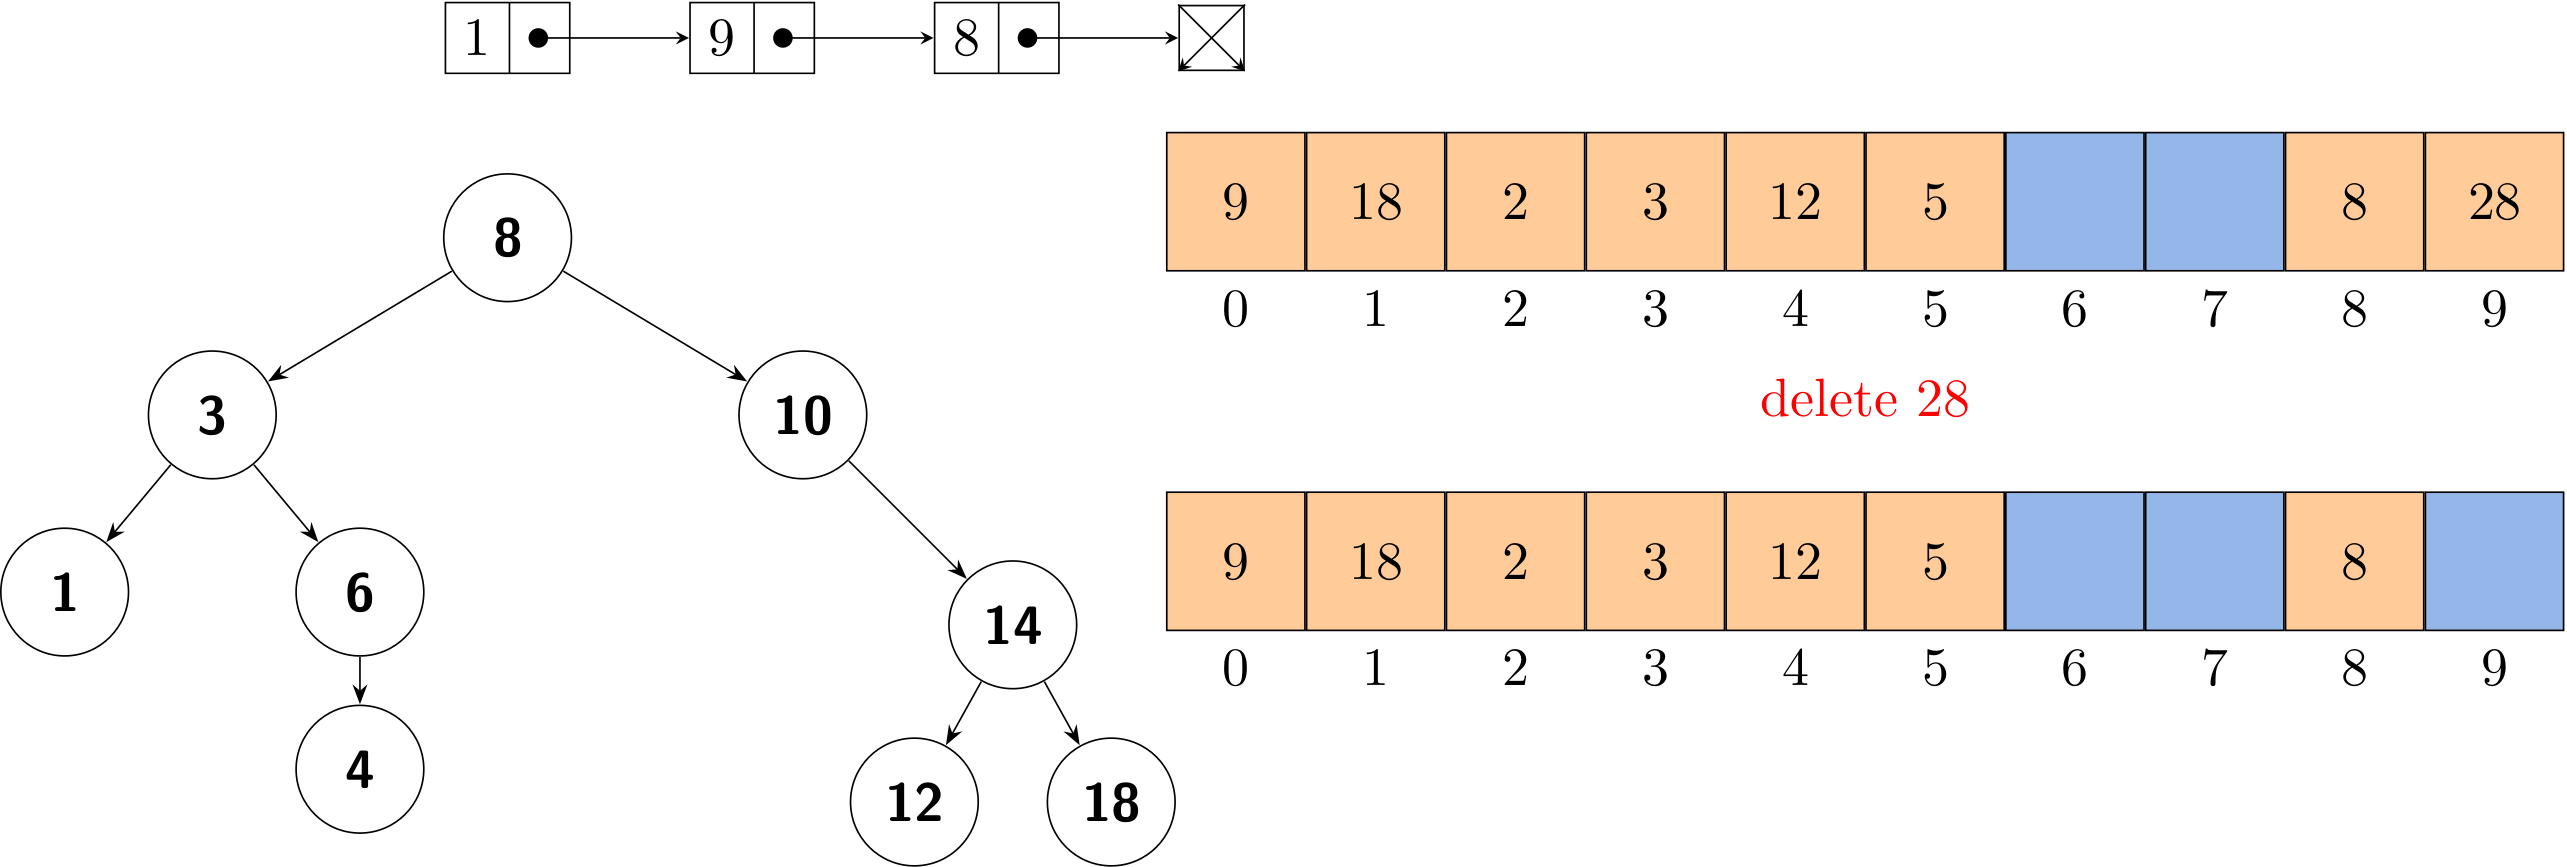
\includegraphics[height=0.7\paperheight]{cover}
    % \end{picture}    
    % }}
    \usebackgroundtemplate{
  \tikz[overlay,remember picture] 
  \node[opacity=0.3, at=(current page.south east),anchor=south east, yshift=2cm,xshift=4cm] {
    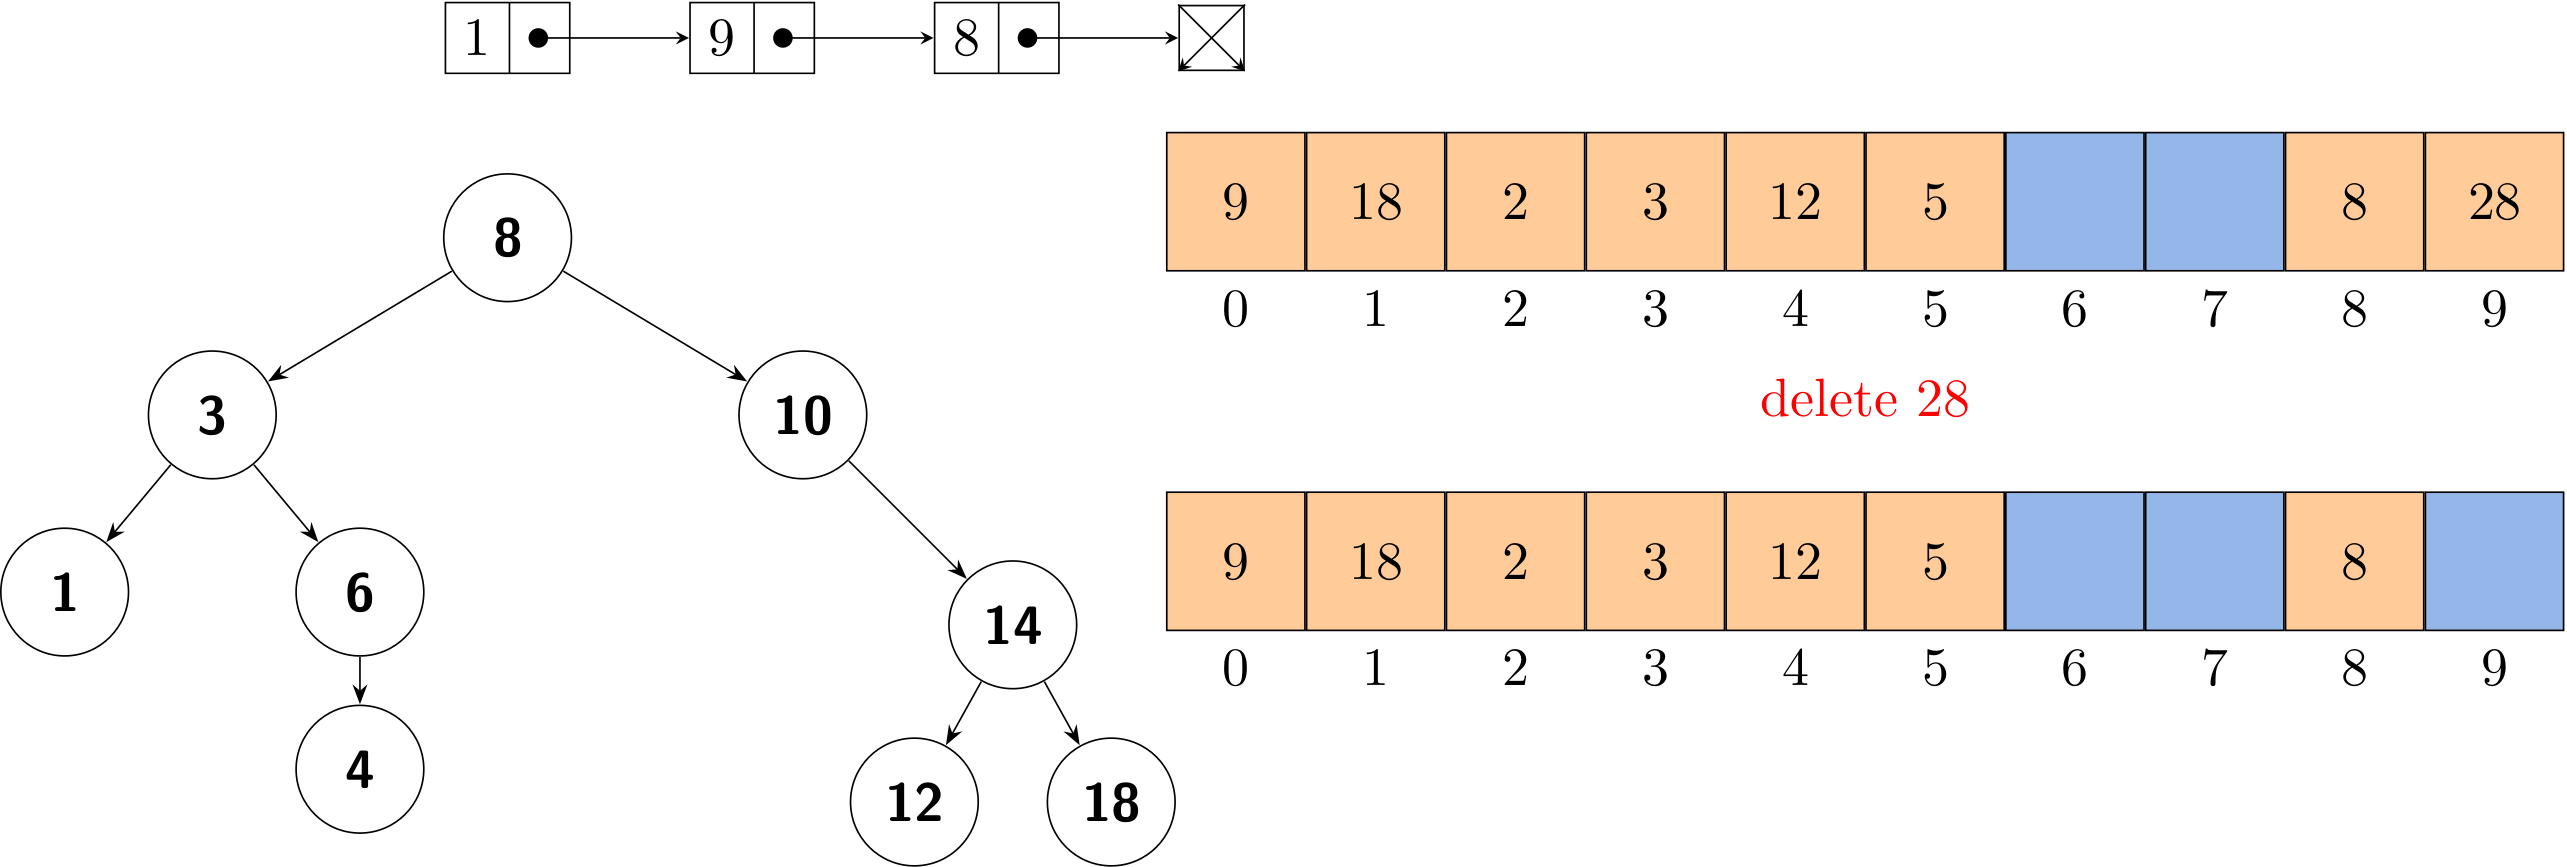
\includegraphics[height=0.6\paperheight]{cover}};
}
    \begin{frame}
        \section{\textcolor{darkmidnightblue}{Course Overview}}
    \end{frame}

}

%---------------------------------------------------------
%Changing visivility of the text


%---------------------------------------------------------
%Example of the \pause command
\begin{frame}[fragile]
\frametitle{About Course}
\begin{exampleblock}{Question}
\textbf{What are \alert{Data Structures}?}
\end{exampleblock}
\pause
\begin{displayquote}
    In computer science, a data structure is a data organization, management, and storage format that is usually chosen for efficient access to data.
\end{displayquote}

\pause

\begin{minted}{java}
List<Book> books = new ArrayList<>();
// add/delete/find book
books.add(new Book("Gone with the wind", 99.0));
\end{minted}

\end{frame}
%---------------------------------------------------------

\begin{frame}[fragile]
    \begin{block}{Fact 1}
        \textbf{Different data structures have varying \alert{capabilities}.}
    \end{block}
    \begin{minted}{java}
String[] books = {"Gone with the Wind", 
"Hands on Data Structures"};
    \end{minted} 
    {\large \faIcon{question-circle}} Can we add a new book onto \emph{books}?
\pause

    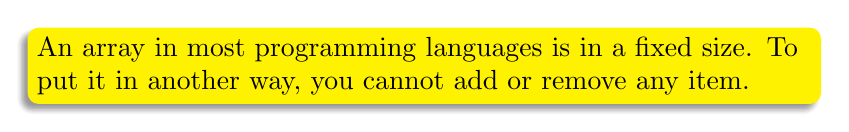
\begin{tikzpicture}
        \node[fill=yellow,blur shadow={shadow xshift=-0.5ex},
        text width=28em,anchor=south west,rounded corners]
        {An array in most programming languages is in a fixed size. To put it in another way, you cannot add or remove any item.};
    \end{tikzpicture} 
\end{frame}

\begin{frame}
    \begin{center}
        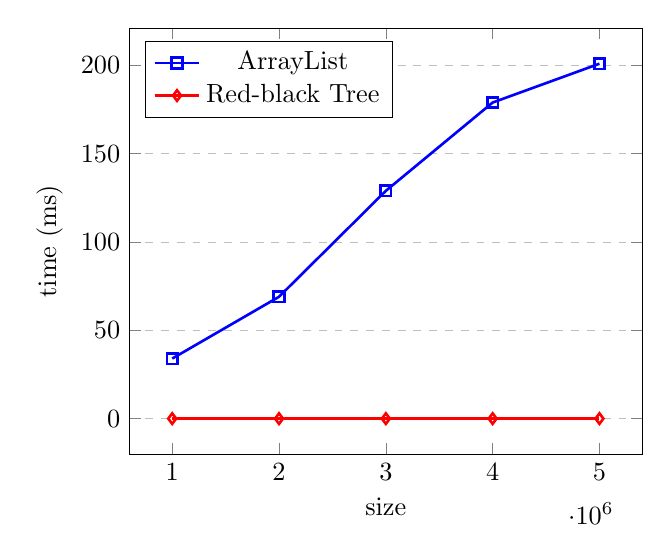
\begin{tikzpicture}[scale=0.95]
            \begin{axis}[
                xlabel={size},
                ylabel={time (ms)},
                ymajorgrids=true,
                grid style=dashed,
                legend pos=north west,
            ]
            \addplot[
                color=blue,
                mark=square,
                line width=1pt,
                ]
                coordinates {
               (1000000, 34)(2000000, 69)(3000000, 129)(4000000, 179)(5000000, 201)
                };
                \addlegendentry{ArrayList}
            
            \addplot[color=red,
            mark=diamond,
            line width=1pt,]
            coordinates {
                (1000000, 0)(2000000, 0)(3000000, 0)(4000000, 0)(5000000, 0)
                 };
            \addlegendentry{Red-black Tree}

            \end{axis}
            \end{tikzpicture}  
    \end{center}
    \begin{block}{Fact 2}
        \textbf{Different data structures have varying \alert{efficiencies}.}
    \end{block} 
\end{frame}

\begin{frame}
    \begin{exampleblock}{Question}
        Suppose there are $10^6$ books in an array. To find a book titled \emph{``Gone with the wind"}, how many times is the comparison performed?
        \begin{enumerate}
            \item On the \textbf{best} case; 
            \item On the \textbf{worst} case; 
            \item On the \textbf{average} case. 
        \end{enumerate}
    \end{exampleblock}
\end{frame}

\begin{frame}
    \begin{center}
        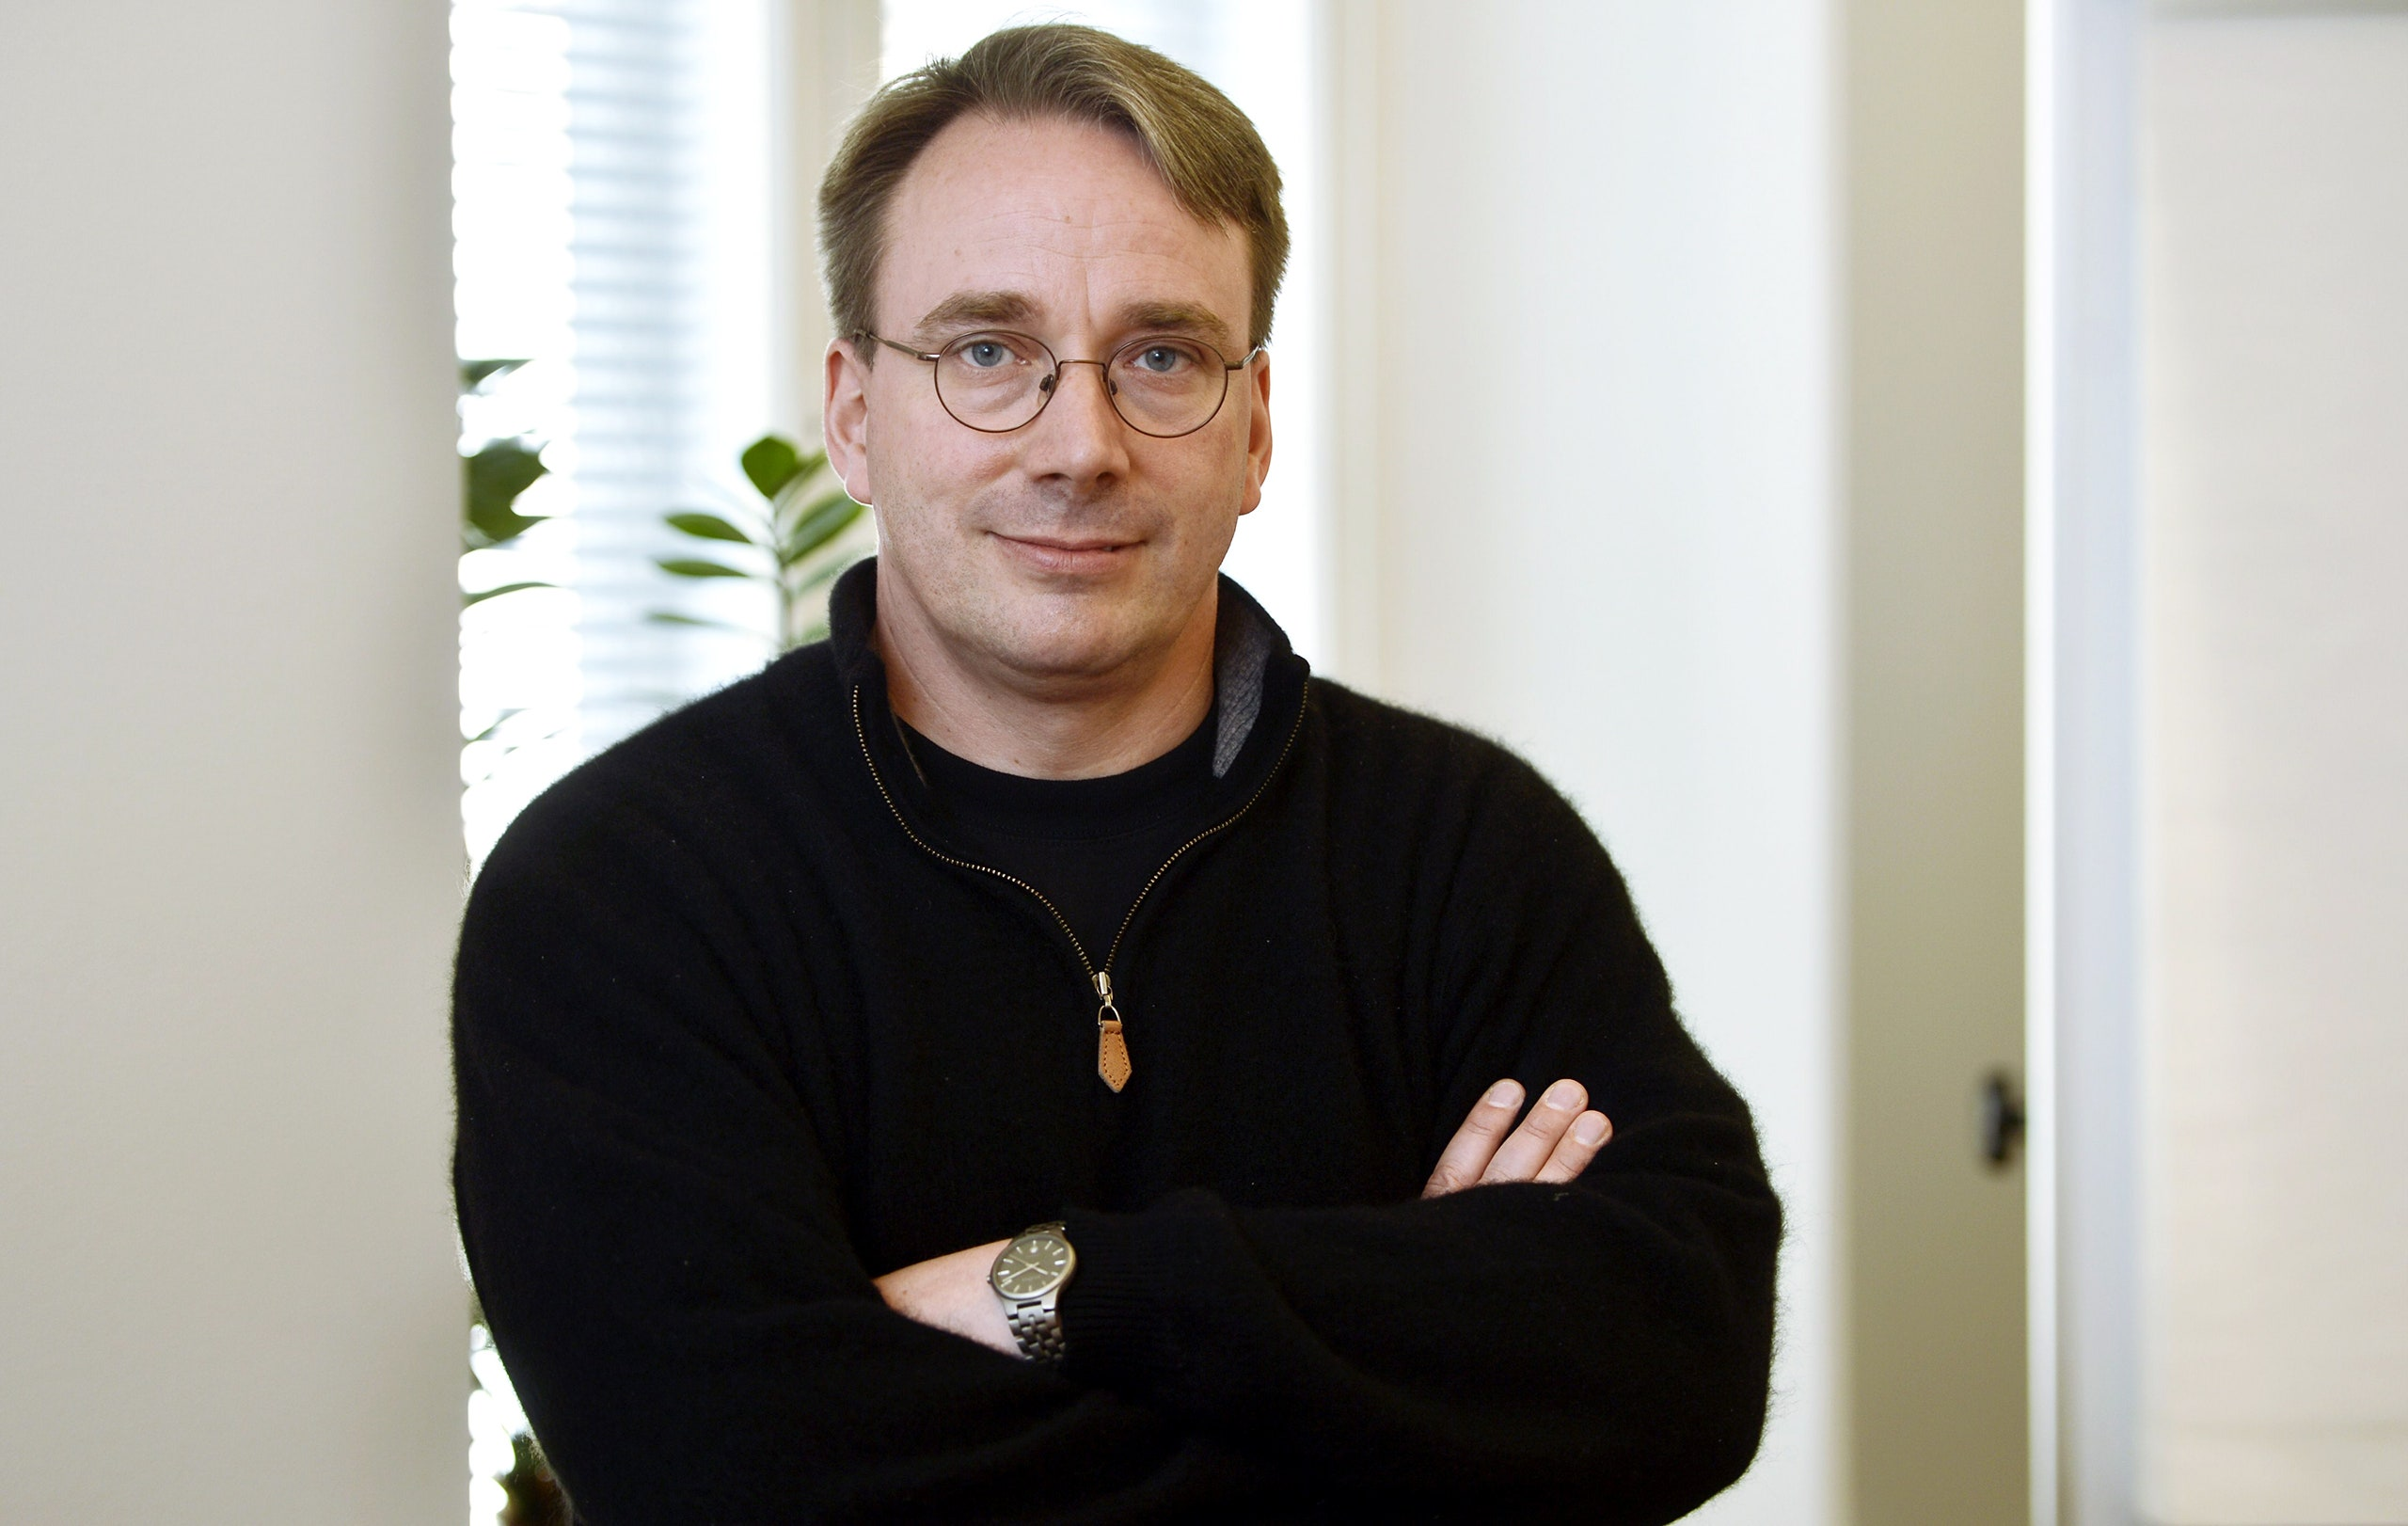
\includegraphics[height=.35\paperheight]{week0/linux}
    \end{center}
    \begin{quote}
        I will, in fact, claim that the difference between a bad programmer and a good one is whether he considers his code or his data structures more important. Bad programmers worry about the code. Good programmers worry about data structures and their relationships.
        \begin{flushright}
            ---Linus Torvalds
        \end{flushright}
    \end{quote}
\end{frame}

\begin{frame}{fragile}
    \frametitle{Algorithm}
    
    $$\mathbf{Data\ Structure + Algorithm = Program}$$

    \begin{quote}
        An algorithm is a finite sequence of rigorous instructions, typically used to solve a class of specific problems or to perform a computation. 
    \end{quote}
\pause
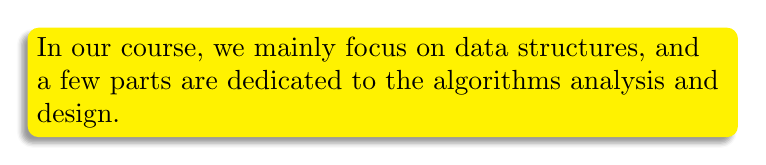
\begin{tikzpicture}
    \node[fill=yellow,blur shadow={shadow xshift=-0.5ex},
    text width=25em,anchor=south west,rounded corners]
    {In our course, we mainly focus on data structures, and a few parts are dedicated to the algorithms analysis and design.};
\end{tikzpicture}

\end{frame}

\begin{frame}
    \frametitle{What you will learn}
    \begin{enumerate}
        \item Language built-in data structures
        \item Stack, queue
        \item Linked list
        \item Balanced search tree
        \item Hash table
        \item Graph
    \end{enumerate}
\end{frame}

\begin{frame}
    \frametitle{Prerequisites and tools}
    \begin{outline}
        \1 Skill of a general (\alert{object-oriented}) programming language (e.g., Python, Java).
        \1 High school level of mathematical skills.
        \1 SDK and IDE
            \2 Java: JDK 11 and above; IntelliJ IDEA 
            \2 Python: Python 3.7 and above; IntelliJ PyCharm
    \end{outline}
    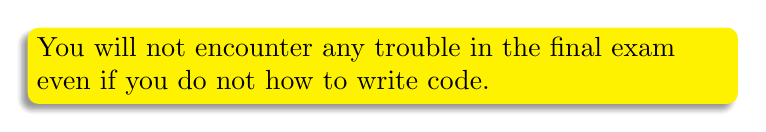
\begin{tikzpicture}
        \node[fill=yellow,blur shadow={shadow xshift=-0.5ex},
        text width=25em,anchor=south west,rounded corners]
        {You will not encounter any trouble in the final exam even if you do not how to write code.};
    \end{tikzpicture} 
\end{frame}

\begin{frame}[fragile]
    \frametitle{Pseudo-code}
    Pseudo\textipa{/"sUdoU/}: not genuine; superficially appears to be one thing, but is something else. 

    \scalebox{.7}{  
        \begin{algorithm}[H]
        \caption{indexOf(a, o)}
        $n\gets a.size()$ \\
        \For{$i\gets 0$ \KwTo $n$}{
            \If{$a[i] == o$}{
                \Return{i}
            }
        }
        \Return{-1}
    \end{algorithm}
    }
\end{frame}

\begin{frame}
    \frametitle{Books}
    \begin{enumerate}
        \item \alert{Introduction to Algorithms} by Thomas H. Cormen, Charles E. Leiserson, Ronald L. Rivest, and Clifford Stein.
        \item \alert{Algorithms} by Robert Sedgewick, Kevin Wayne.
        \item \alert{Data Structures and Algorithms in Java} by Michael T. Goodrich, Roberto Tamassia, Michael H. Goldwasser.
        \item \alert{Data Structures and Algorithms in Python} by Michael T. Goodrich, Roberto Tamassia, Michael H. Goldwasser.
    \end{enumerate}
    \pause
    \textbf{\href{https://chenzhongpu.github.io/data-structure-swufe/}{Hands On Data Structures}} by me.
\end{frame}

\begin{frame}
    \begin{figure}
        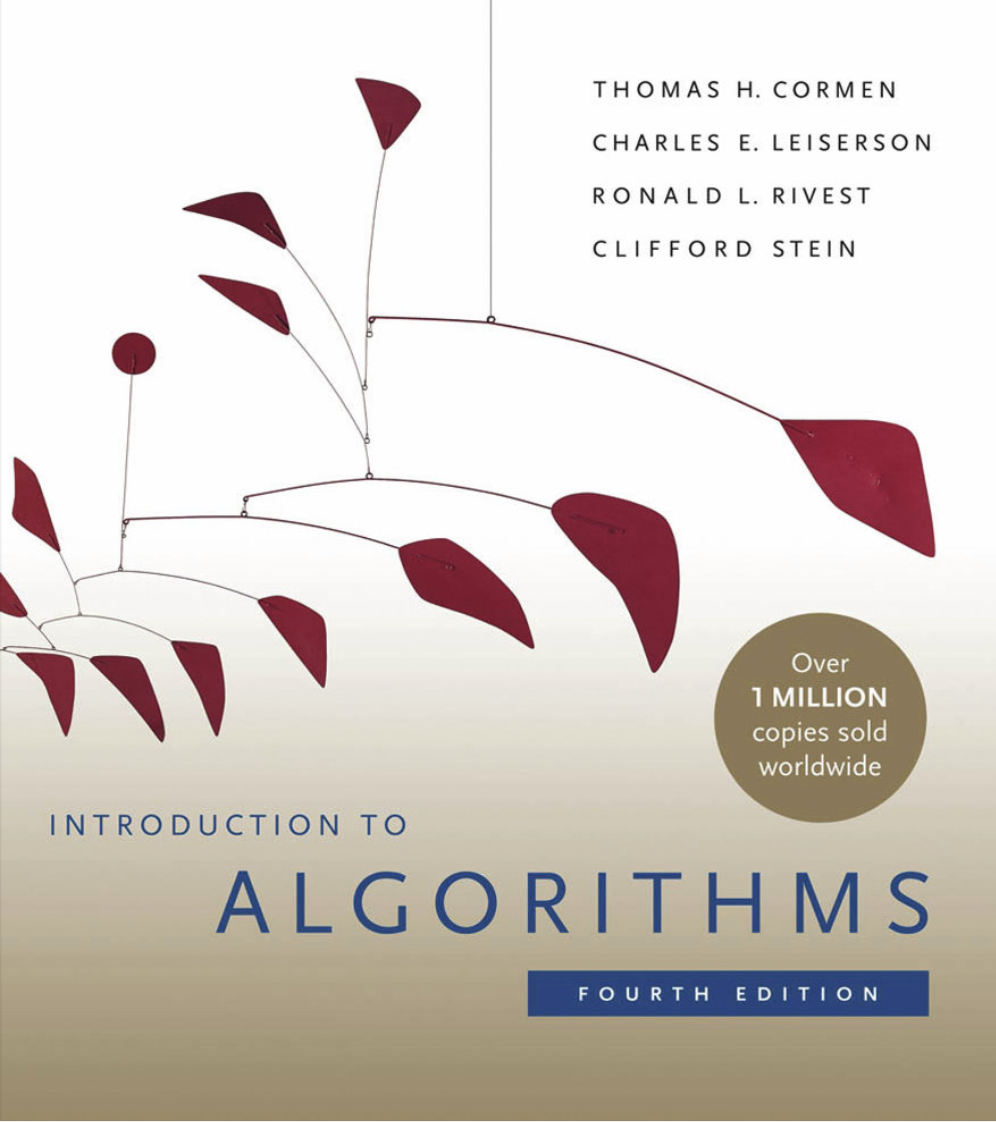
\includegraphics[width=0.475\textwidth]{week0/intro-to-alg}
        \hfill
        
\includegraphics[width=0.475\textwidth]{week0/algs4}
    \end{figure} 
\end{frame}

\begin{frame}
    \frametitle{Resources}
    \begin{itemize}
        \item Course (slides and syllabus) @\href{https://zhongpu.info/teaching/cs906-2022-fall}{zhongpu.info}
        \item Code@\href{https://github.com/ChenZhongPu/data-structure-swufe}{GitHub}
        \item Book@\href{https://chenzhongpu.github.io/data-structure-swufe/}{GitHub}
        \item Online discussion@Feishu Group
    \end{itemize}
    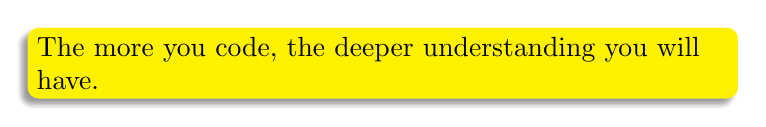
\begin{tikzpicture}
        \node[fill=yellow,blur shadow={shadow xshift=-0.5ex},
        text width=25em,anchor=south west,rounded corners]
        {The more you code, the deeper understanding you will have.};
    \end{tikzpicture}
\end{frame}

\begin{frame}
    \frametitle{Assessment}
    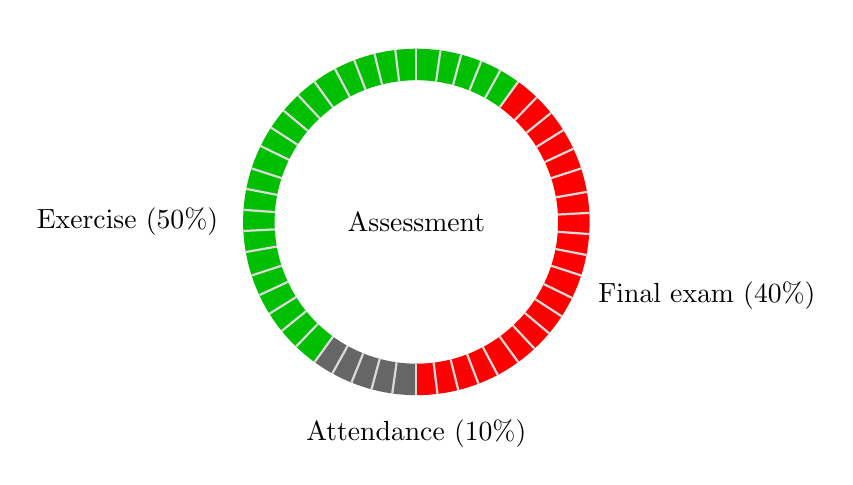
\begin{tikzpicture}
        \colorlet{good}{green!75!black}
        \colorlet{bad}{red}
        \colorlet{neutral}{black!60}
        \colorlet{none}{white}
      
        \node[align=center,text width=3cm]{Assessment};
      
        \begin{scope}[line width=4mm,rotate=270]
          \draw[good]          (144:2cm) arc (144:324:2cm);
          \draw[neutral]       (-36:2cm) arc (-36:0:2cm);
          \draw[bad]  (0:2cm)  arc (0:144:2cm);
      
          \newcount\mycount
          \foreach \angle in {0,72,...,3599}
          {
            \mycount=\angle\relax
            \divide\mycount by 10\relax
            \draw[black!15,thick] (\the\mycount:18mm) -- (\the\mycount:22mm);
          }
      
          \draw (0:2.2cm) node[below] {Attendance (10\%)};
          \draw (-90:2.2cm) node[left] {Exercise (50\%)};
          \draw (65:2.2cm) node[right] {Final exam (40\%)};
        \end{scope}
        % \draw[gray] (0,0) circle (2.2cm) circle (1.8cm);
      \end{tikzpicture}
      
\begin{tikzpicture}
        \node[fill=red!80, text=white, blur shadow={shadow xshift=-0.5ex},
        text width=15em,anchor=south west,rounded corners, ]
        {Plagiarism is strictly prohibited!
        };
      \end{tikzpicture}
\end{frame}

\section{\textcolor{darkmidnightblue}{A Few Notes on Languages}}

\begin{frame}
    \begin{center}
        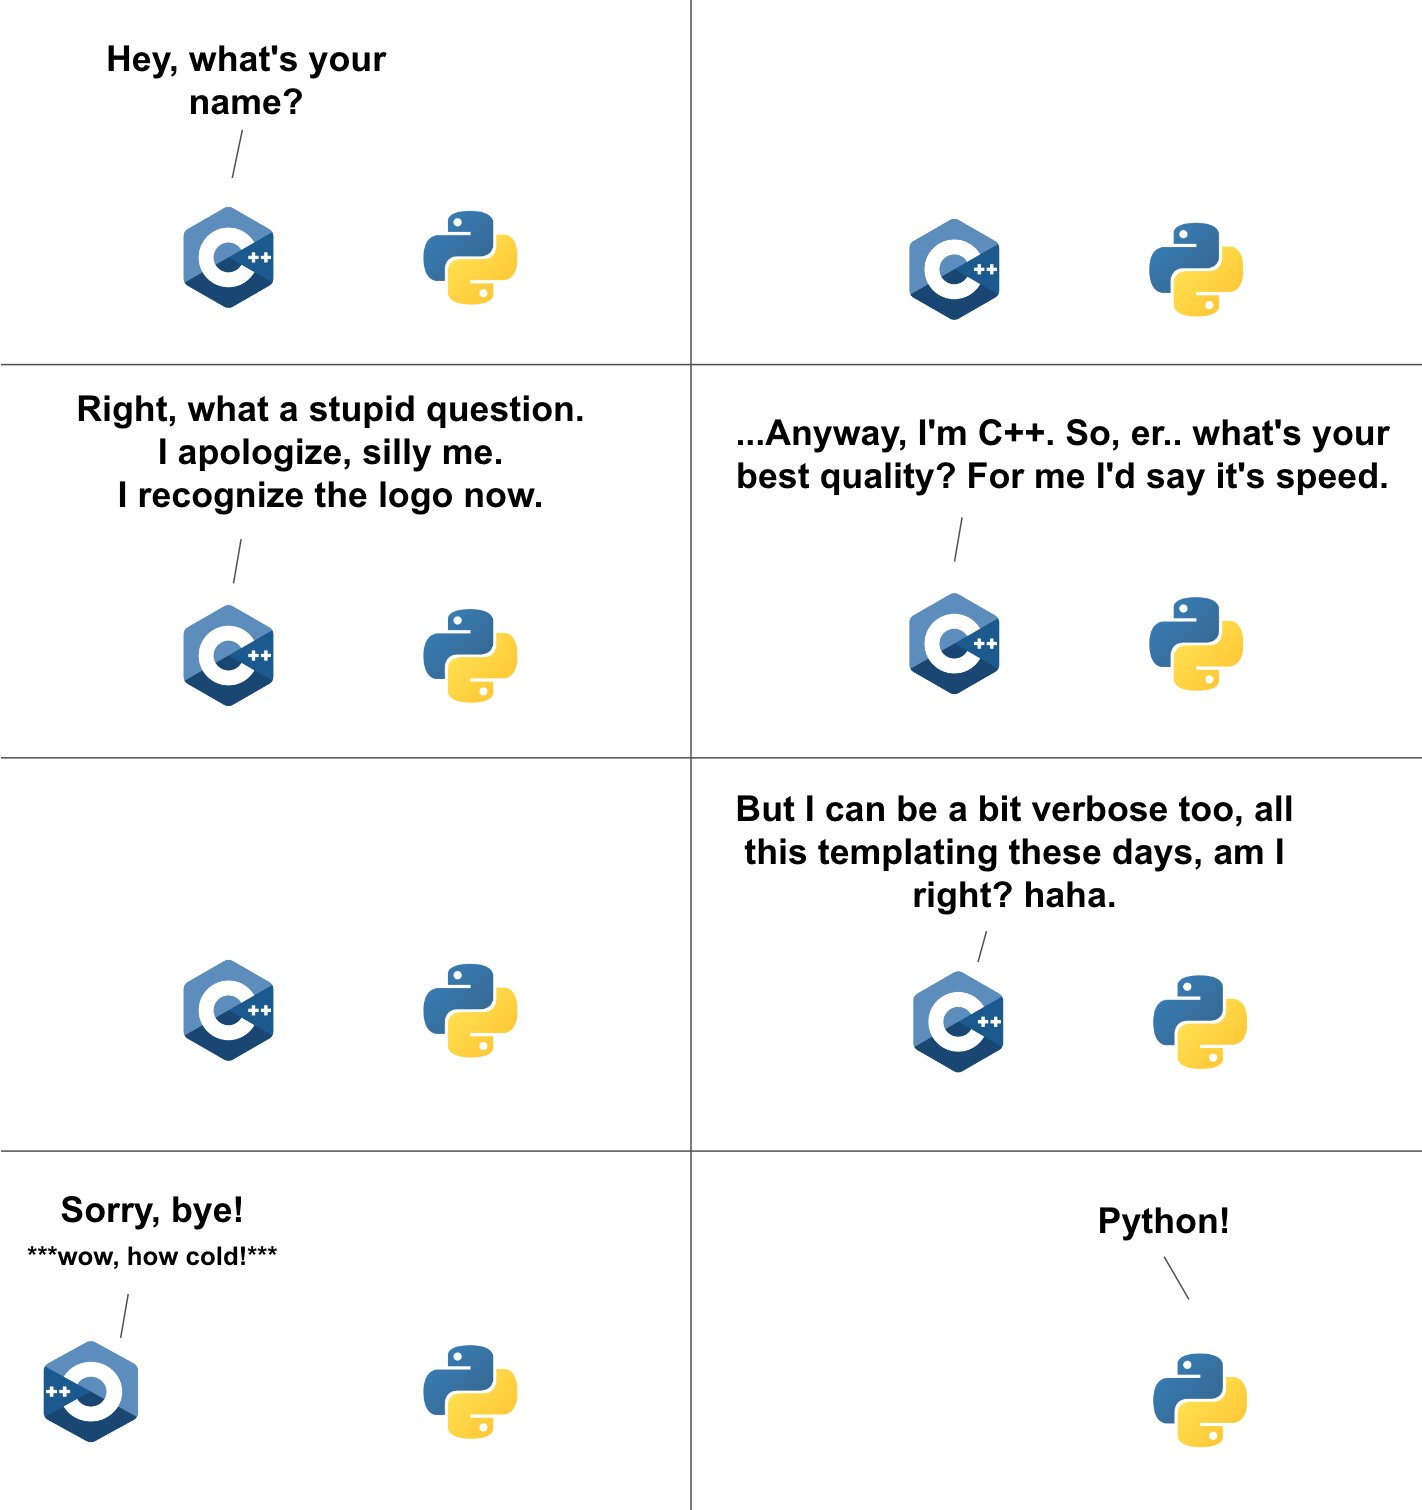
\includegraphics[height=.95\paperheight]{week0/py-c++}
    \end{center}
\end{frame}

\begin{frame}
    \begin{center}
        
\includegraphics[height=.95\paperheight]{week0/py}
    \end{center}
\end{frame}

\begin{frame}{Python vs. Java}
    \begin{table}
        \caption{Comparison table}
        \begin{tabular}{lr}
          \toprule
          Python & Java\\
          \midrule
          Interpreted language & Compiled language\\
          Dynamically typed & Statically typed\\
          Slightly more popular & Less popular\\
          Less code & More code\\
          Much Slower & Much faster \\
          Hard to maintain & Higher stability \\
          \bottomrule
        \end{tabular}
    \end{table}
\end{frame}

\begin{frame}[fragile]
    \begin{columns}
        \column{0.45\textwidth}
        Python:
        \begin{minted}{python}
            i = 42
            i = 'data'
        \end{minted}
    
        \column{0.45\textwidth}
          Java:
          \begin{minted}{java}
            int i = 42;
            i = "data";
        \end{minted}
      \end{columns}
\end{frame}

\begin{frame}[fragile]
    \frametitle{Python's Fibonacci}
    \begin{minted}[bgcolor=LightGray]{python}
def fibonacci(n):
    if n == 0:
        return 0
    elif n == 1 or n == 2:
        return 1
    else:
        return fibonacci(n - 1) + fibonacci(n - 2)        
    \end{minted}
\end{frame}

\begin{frame}[fragile]
    \frametitle{Java's Fibonacci}
    \begin{minted}[bgcolor=LightGray]{java}
public long fibonacci(int n) {
    if (n == 0) {
        return 0;
    } else if (n == 1 || n == 2) {
        return 1;
    } else {
        return fibonacci(n - 1) + fibonacci(n - 2);
    }
}    
    \end{minted}
\end{frame}

\end{document}